\section{Physical Connections and Interfaces}

`v2 sensor boards' means a set of sensors which includs a v2.08 Airsense board, a v2 Lightsense board, and a Chemsense board.
\par
Physical connections between sensor boards and sensors are shown in the Figure \ref{fig:physicalConnections}. Airsense board is connected to lightsense board through CAT6 cable, and chemsense board is connected to lightsense board through jumper cables. Airsense and lightsense deliver data through I2C communication, and chemsense board delivers data through serial3 communication. All sensor data from airsense, lightsense, and chemsense board are delivered to nodecontroller thourgh converter cable attached on airsense board using I2C communication.
\par
Four pins on the Metsense board and the Chemsense board need to be connected in the order located as shown in the Figure \ref{fig:physicalConnections} through jumpers. This means that each of the pin at the right end need to be connected, and the same to all the other pins. The left end pin of each board is ground.
\\

\begin{figure}[h]
\begin{center}
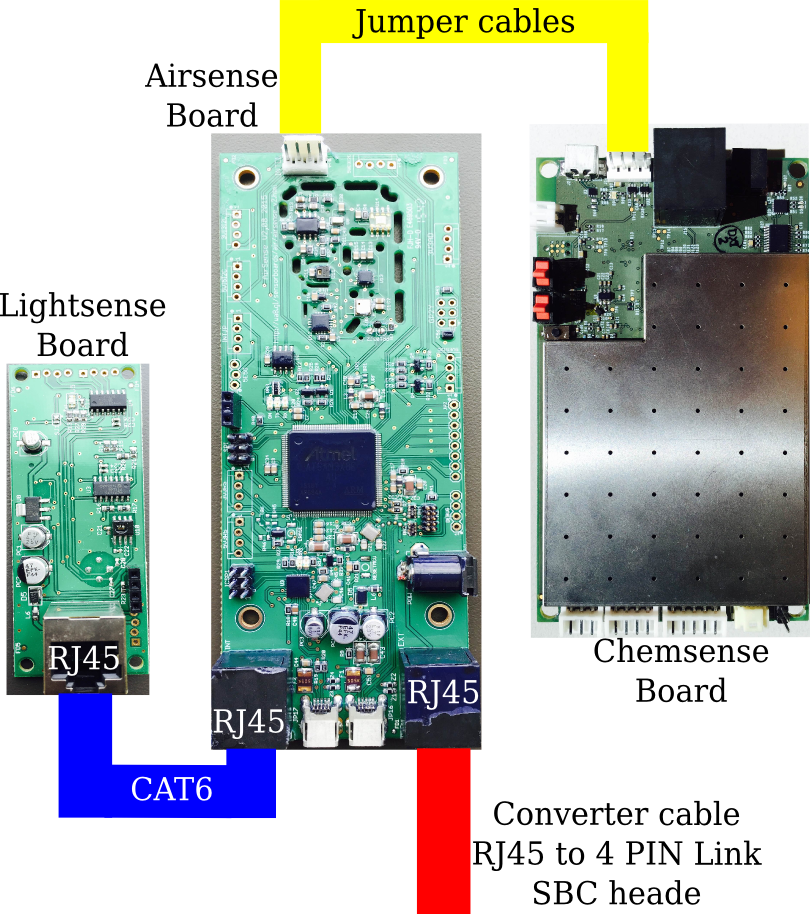
\includegraphics[width=4in]{g4353.png}
\caption{Connections between the sensor boards and the sensor}
\label{fig:physicalConnections}
\end{center}
\end{figure}

